\documentclass{standalone}
\usepackage{tikz}

\begin{document}

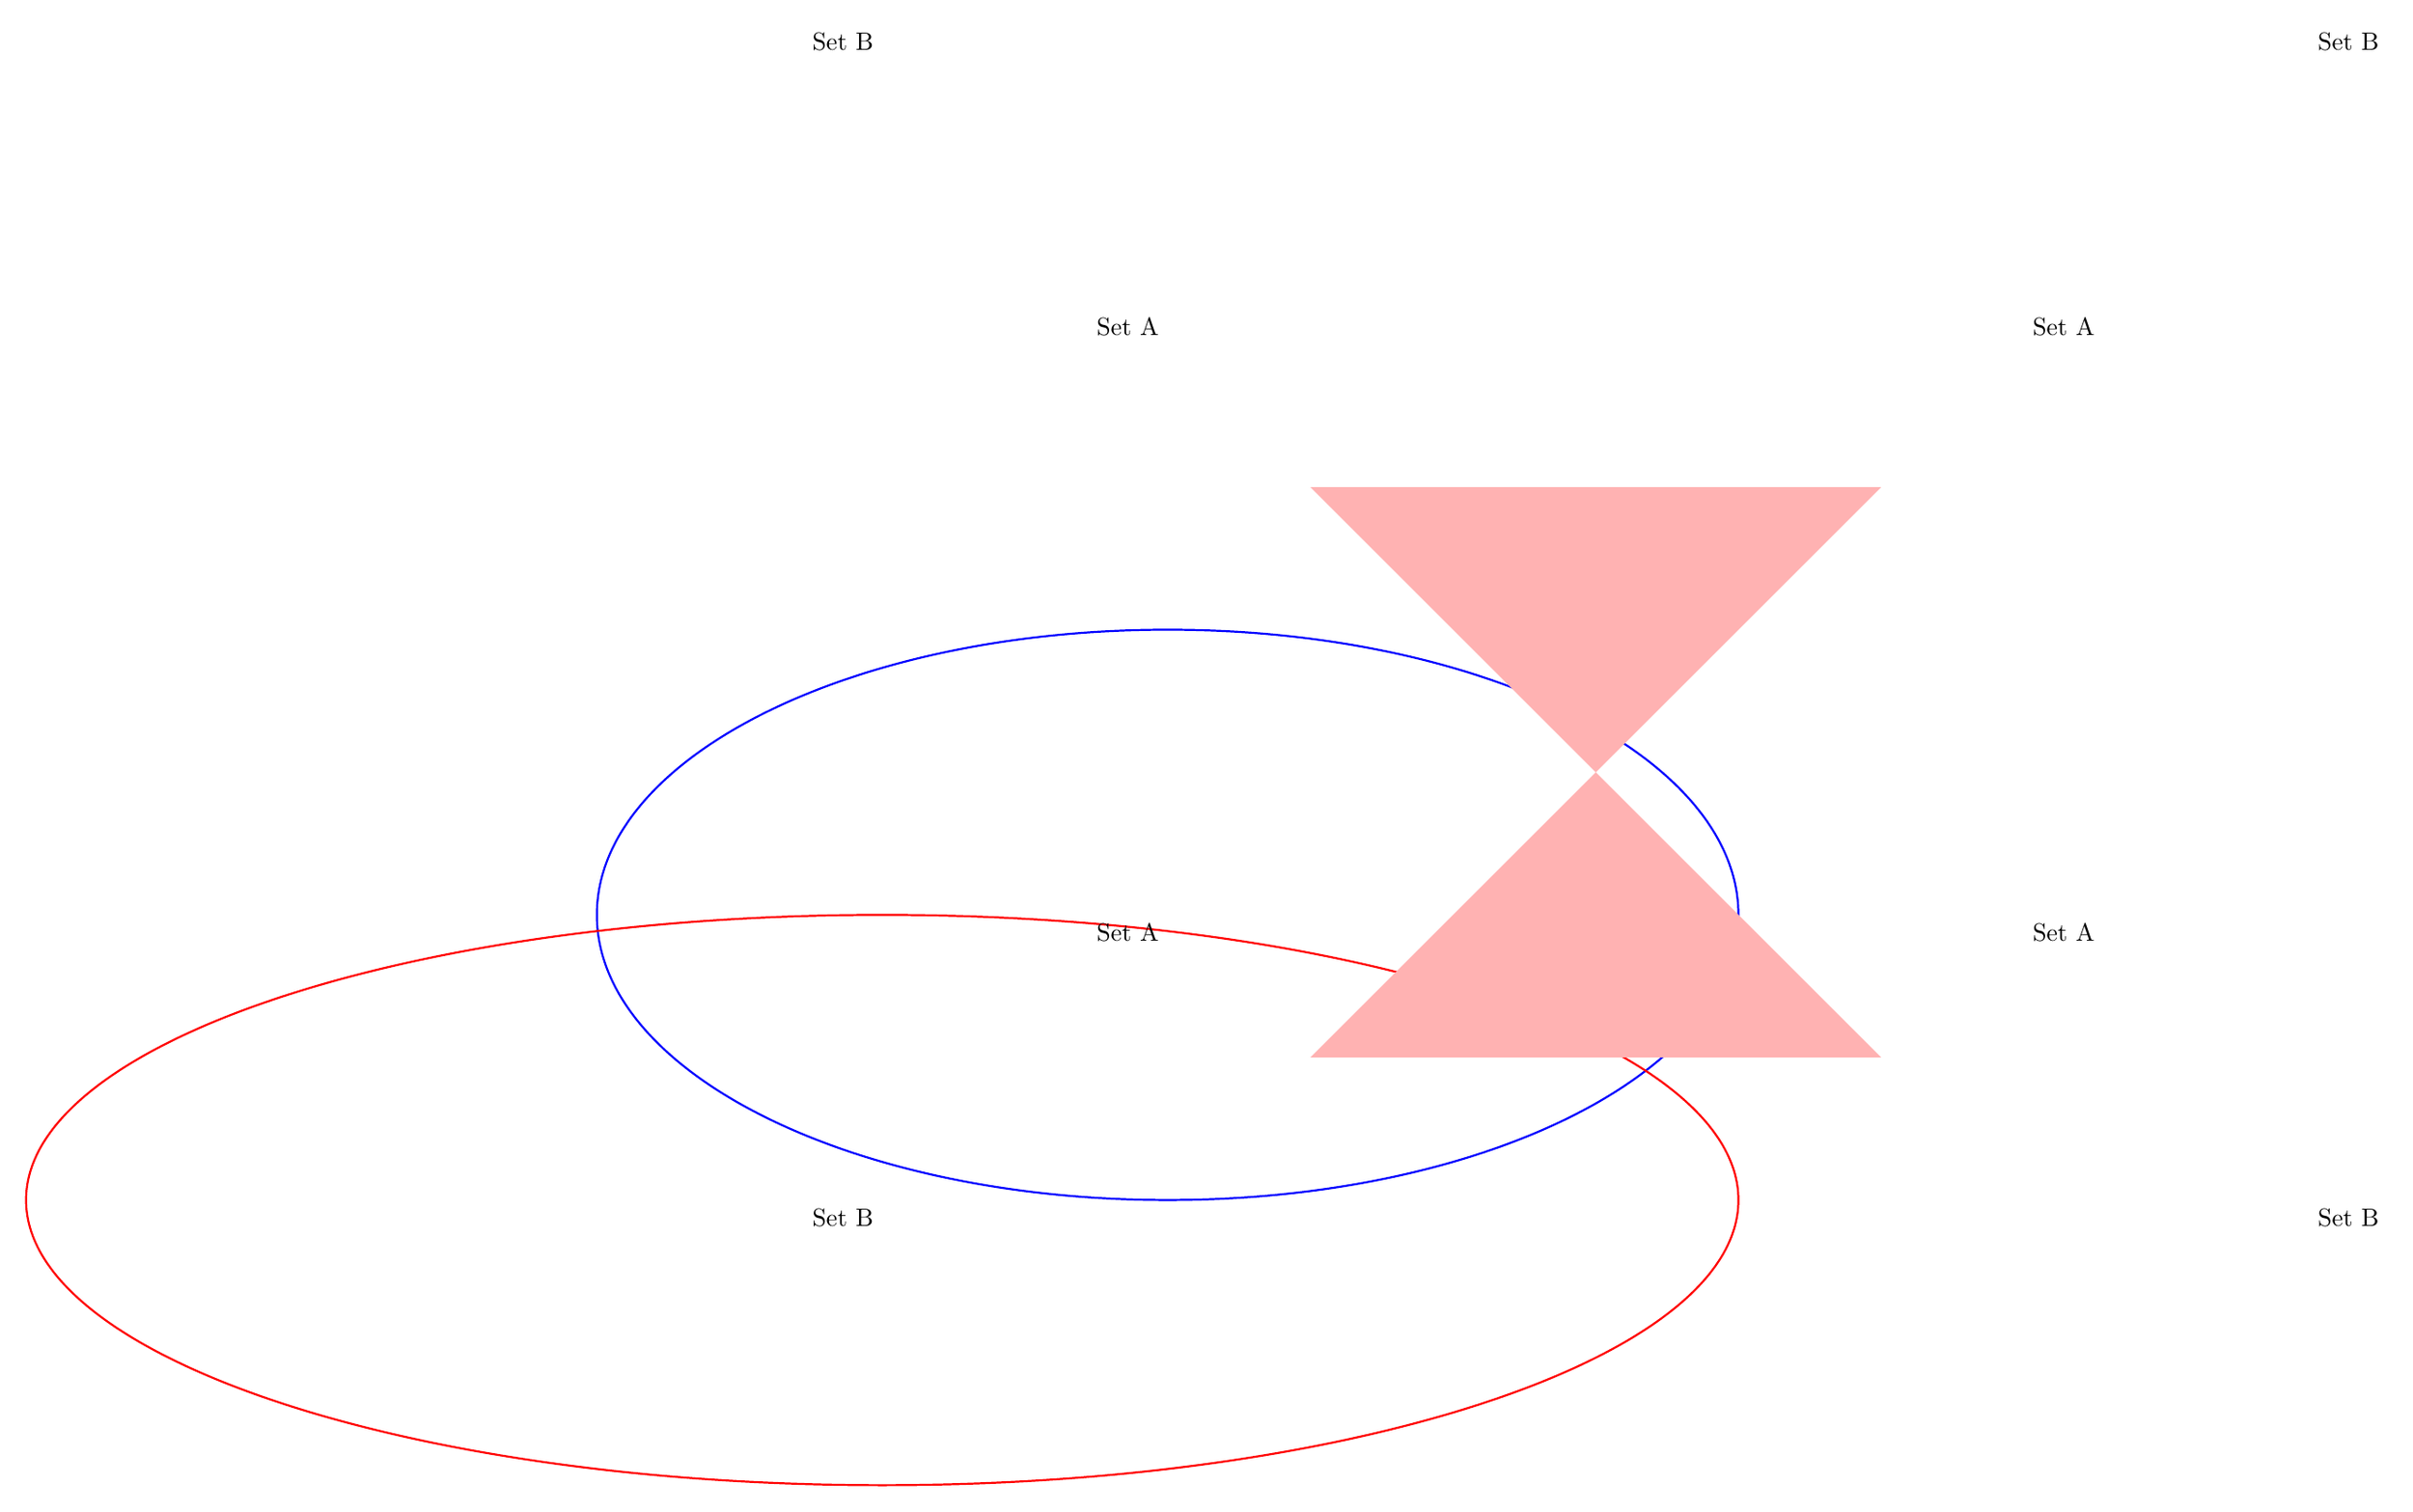
\begin{tikzpicture}[scale=2]

% Define coordinates for the first circle
\coordinate (A1) at (-3,-1);
\coordinate (A2) at (3,-1);
\coordinate (A3) at (-3,3);
\coordinate (A4) at (3,3);

% Define coordinates for the second circle
\coordinate (B1) at (-5,-3);
\coordinate (B2) at (5,-3);
\coordinate (B3) at (-5,5);
\coordinate (B4) at (5,5);

% Draw the first circle
\draw[thick, blue] (A1) ellipse[x radius=4, y radius=2];

% Draw the second circle
\draw[thick, red] (B1) ellipse[x radius=6, y radius=2];

% Define coordinates for the intersection region
\coordinate (C1) at (-2,-2);
\coordinate (C2) at (2,-2);
\coordinate (C3) at (-2,2);
\coordinate (C4) at (2,2);

% Draw the irregularly shaped overlap
\fill[blue!30,red!30] (C1) -- (C2) -- (C3) -- (C4) -- cycle;

% Add labels
\node[below left] at (A1) {Set A};
\node[below right] at (A2) {Set A};
\node[above left] at (A3) {Set A};
\node[above right] at (A4) {Set A};

\node[below left] at (B1) {Set B};
\node[below right] at (B2) {Set B};
\node[above left] at (B3) {Set B};
\node[above right] at (B4) {Set B};

\end{tikzpicture}

\captionof{figure}{Perfectly balanced Venn diagram with uneven circle shapes.}

\end{document}